\chapter{Desarrollo de la aplicación}

\epigraph{\textit{''Los programas deben ser escritos para que los lean las personas, y sólo incidentalmente, para que lo ejecuten las máquinas''}}{--- Abelson and Sussman}

Tras haber explicado en el capítulo anterior las diversas herramientas a usar para el desarrollo de la aplicación, en este capítulo se explicaran aspectos sobre el diseño de la aplicación y las diferentes decisiones tomadas a la hora de realizar dicho diseño.

El diseño de la aplicación es simple y minimista. El objetivo del proyecto consiste en hacer una aplicación lo más fácil de usar y con la mayor claridad posible de cara al usuario. Por ello, se ha optado por un enfoque que reduzca el numero de elementos al mínimo, además de que se adapta perfectamente a los estándares de diseño de Material Design\footnote{\url{https://material.io/design/}}, que son los recomendados a la hora de diseñar aplicaciones para Android.

\section{Interfaz gráfica}

Para la interfaz gráfica se ha optado por hacer un diseño inicial en papel para después, en base a ese diseño y esa distribución de ventanas, elaborar en Android Studio toda la interfaz gráfica. Se puede observar un diseño primitivo en la siguiente imagen.

\begin{figure}[ht]
	\centering
	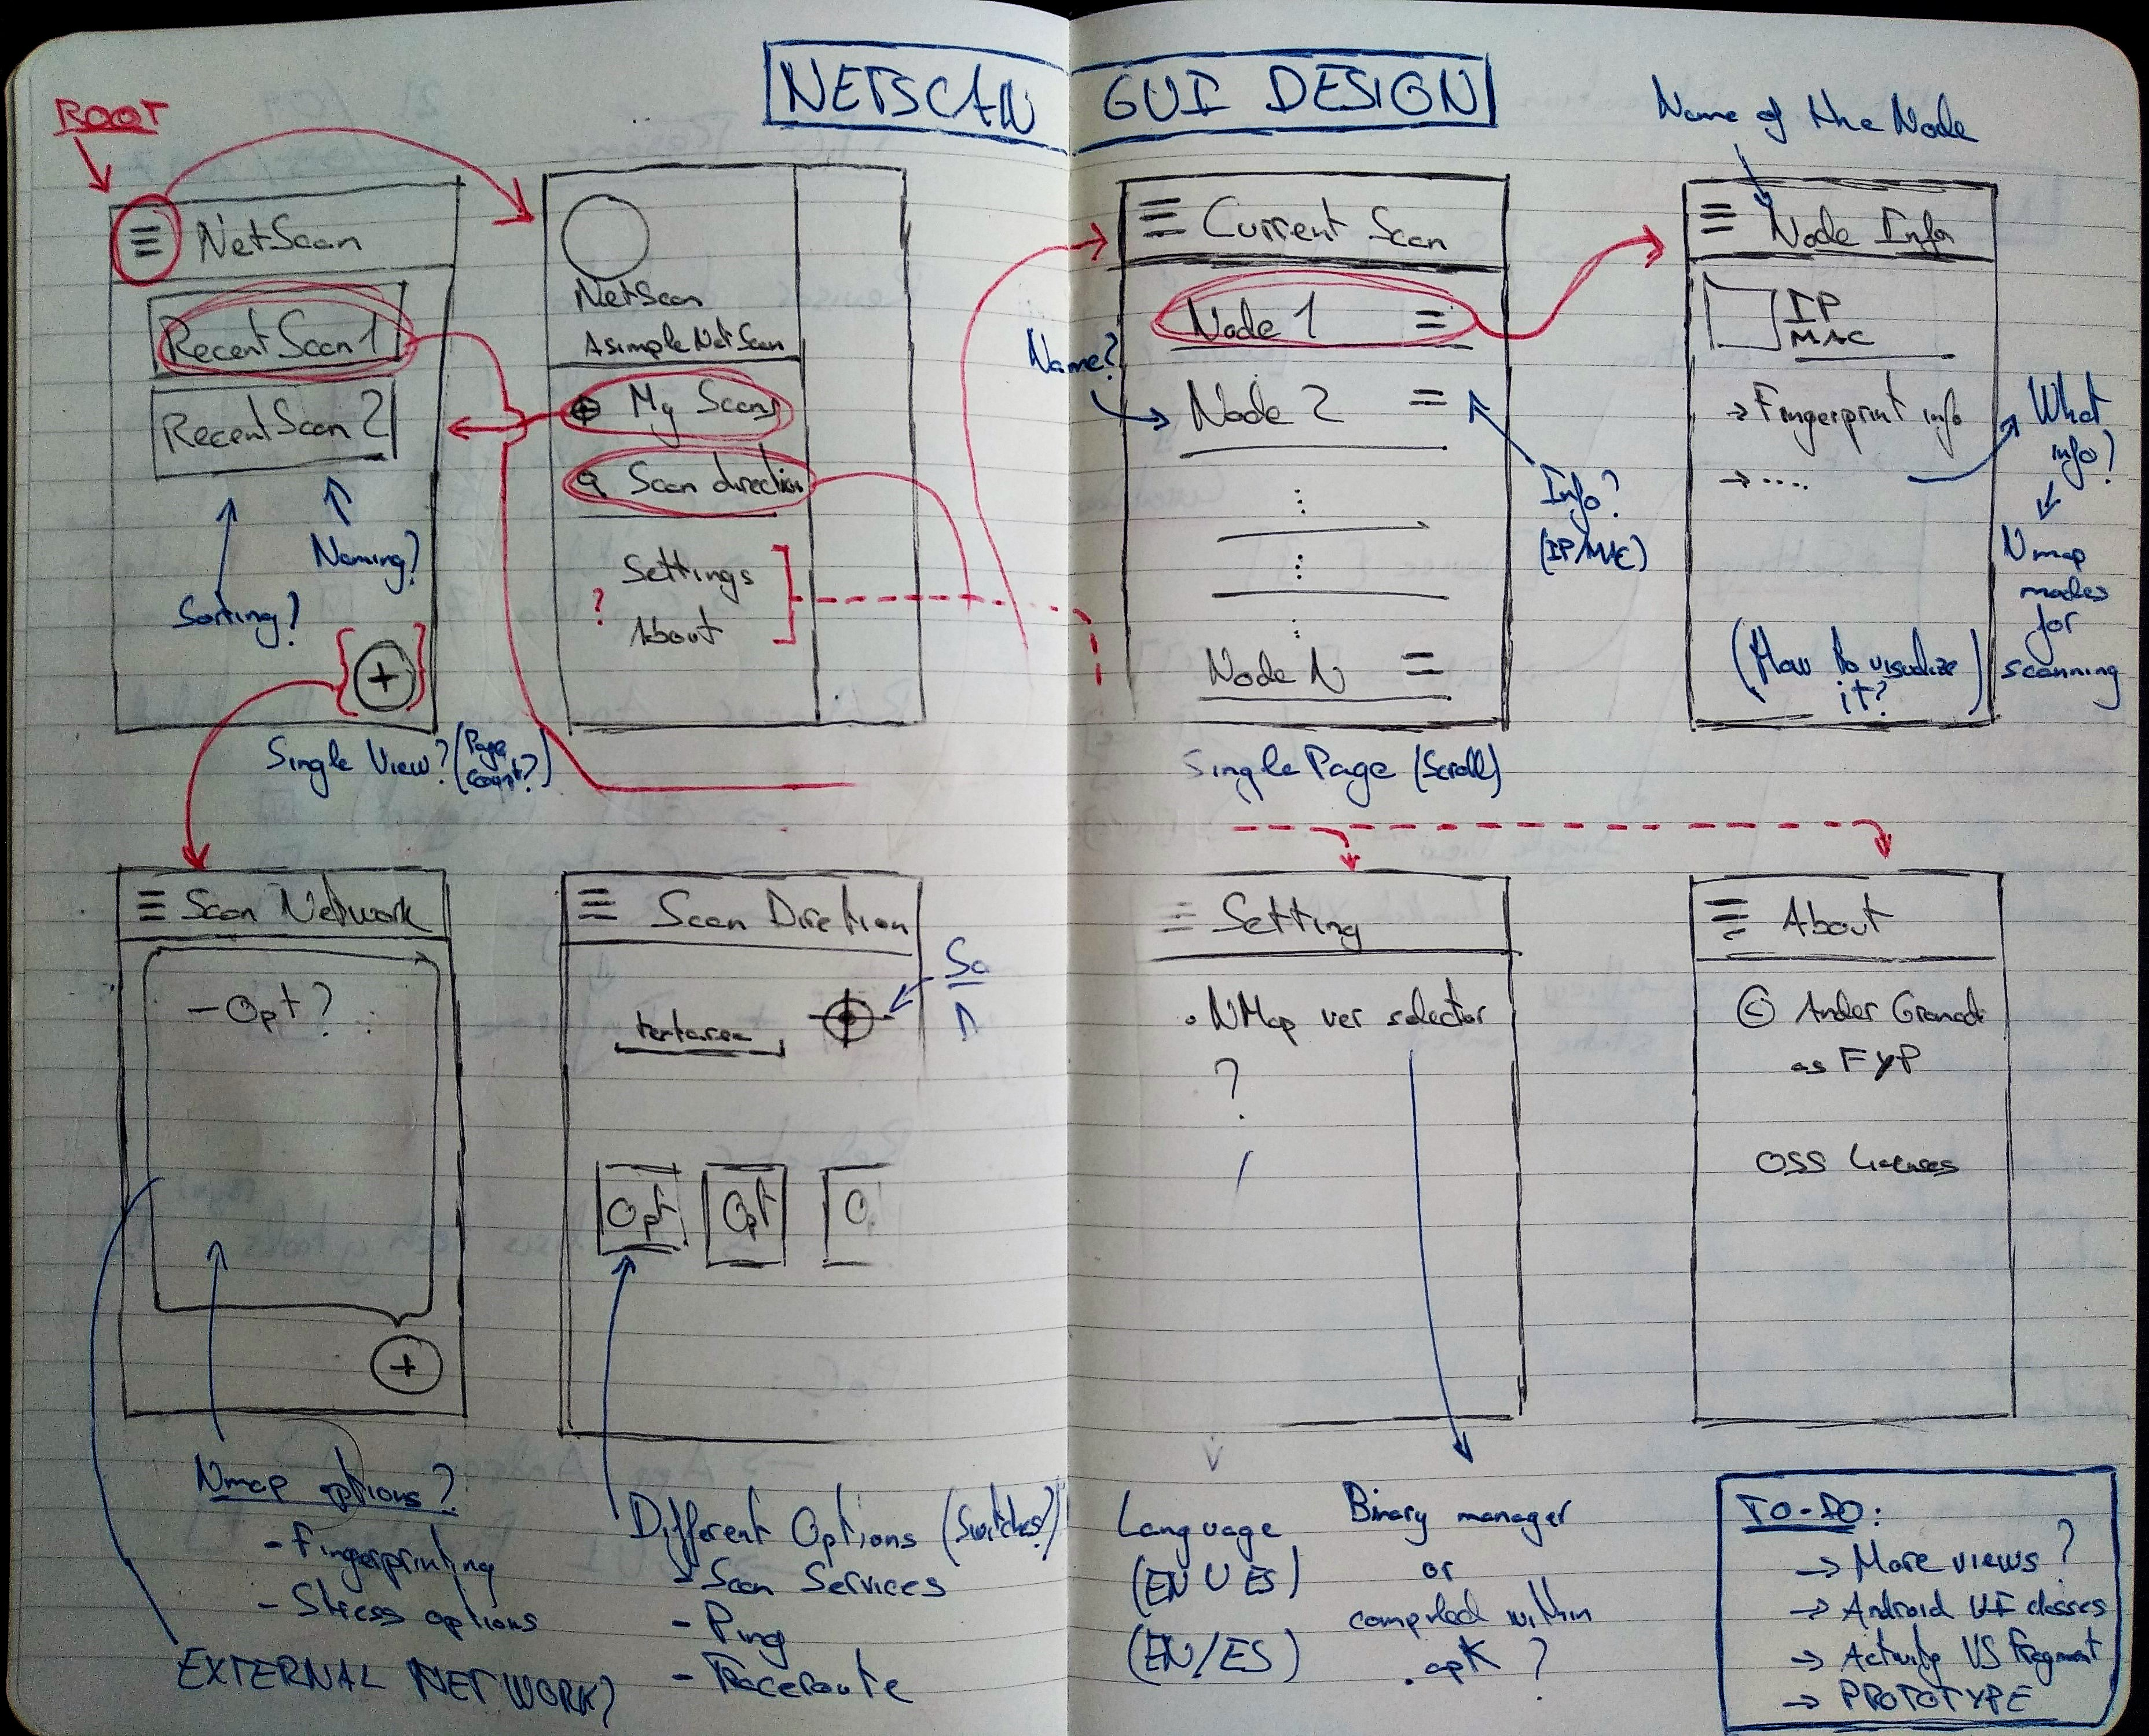
\includegraphics[width=\textwidth]{gui-mockup}
	\caption{Mockup inicial de la GUI de la aplicación}
	\label{fig:mockup}
\end{figure}

La aplicación esta dividida en varias vistas. Debido a que el objetivo principal de la aplicación es que sea lo mas simple posible, se ha diseñado buscando minimizar el numero de ventanas de la aplicación.

A la hora de crear las vistas en Android se usan dos conceptos. \textit{Activity} y \textit{Fragment}. En Android, una Activity representa una parte de la UI de una aplicación, y tiene su propio ciclo de vida y su propia jerarquía de elementos. Una aplicación Android dispone de tantas Activity como el usuario quiera implementar, entendiendo que cada Activity servirá para mostrar cierta información e interactúa con el usuario de una manera concreta. En términos genéricos, equivale a una vista concreta de una aplicación. Los aspectos mas técnicos se abordarán durante la explicación de la implementación.

El Fragment, aunque también representa una parte de la UI de la aplicación, depende de una Activity, ya que debe acoplarse a una. A diferencia del Activity, se pueden mostrar varios Fragments a la vez. Hay que tener en cuenta que un Fragment, aun teniendo su propio ciclo de vida (más simplificado que el del Activity) depende del ciclo de vida del Activity al que este acoplado. 

En Android, a la hora de diseñar aplicaciones, se usan Fragments para partes reutilizables y comunes de una UI y se usan las Activities para controlar el ciclo de vida de la aplicación. En una aplicación de Android abierta siempre se encuentra activa una Activity, que muestra algún tipo de interfaz.

La aplicación dispone de una serie Activities y Fragments implementados, cuya lista se muestra en la \autoref{fig:views-list}.

\begin{figure}[t]
	\centering
	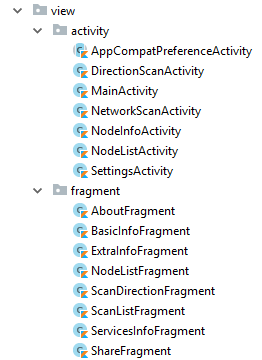
\includegraphics{views-list}
	\caption{Lista de clases con las Activities y Fragments implementados en la aplicación}
	\label{fig:views-list}
\end{figure}

Cómo se puede observar en la imagen existen una serie de Activities y Fragments que sirven para implementar las diferentes ventanas basándose en ese primer y primitivo diseño de la interfaz. Se observa que también existen más elementos que los correspondientes a las vistas inicialmente diseñadas. A medida que se ha ido desarrollando la aplicación, y en función de las necesidades de la funcionalidad, se han ido añadiendo más elementos. Este diseño de Activities y Fragments corresponde al diseño final de la aplicación.

\section{Navegación}

A la hora de programa de una interfaz gráfica, una de las cosas que debemos tener en cuenta es el flujo de interacción entre las diferentes vistas. Esto consiste en entender que vistas interactúan con otras, es decir, el proceso que sigue el usuario para llegar a una u otra ventana concreta. A esto se conoce como \textit{flujo} de la aplicación. El flujo de la aplicación es bastante sencillo coma y se muestra en la \autoref{fig:flow-diagram}

\begin{figure}[H]
	\centering
	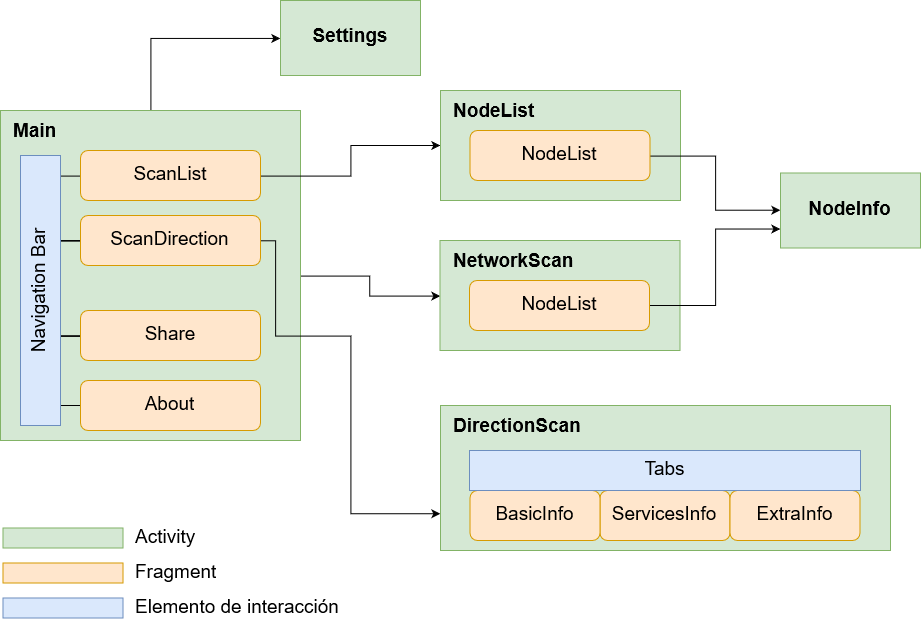
\includegraphics[width=\textwidth]{flow-diagram}
	\caption{Diagrama de flujo entre los diferentes elementos de la interfaz}
	\label{fig:flow-diagram}
\end{figure}

El diagrama muestra claramente cómo interactúan los diferentes Activities y Fragments.  Como se puede apreciar, la aplicación parte de un punto, de una Activity concreta, llamada \textbf{MainActivity}. Esta Activity es la que arrancará al iniciarse la aplicación. Dentro de ella, tenemos cuatro posibles Fragments a mostrar. Cuál se mostrará dependerá de la opción seleccionada en una barra de navegación lateral, o \textit{Navbar}. Por defecto está seleccionada la opción \textbf{ScanListFragment}. Accediendo a esa barra de navegación cambiamos entre un menú u otro, implementado en un Fragment u otro. Se puede ver el diseño de la barra de navegación en la \autoref{fig:navbar}

\begin{figure}[H]
	\centering
	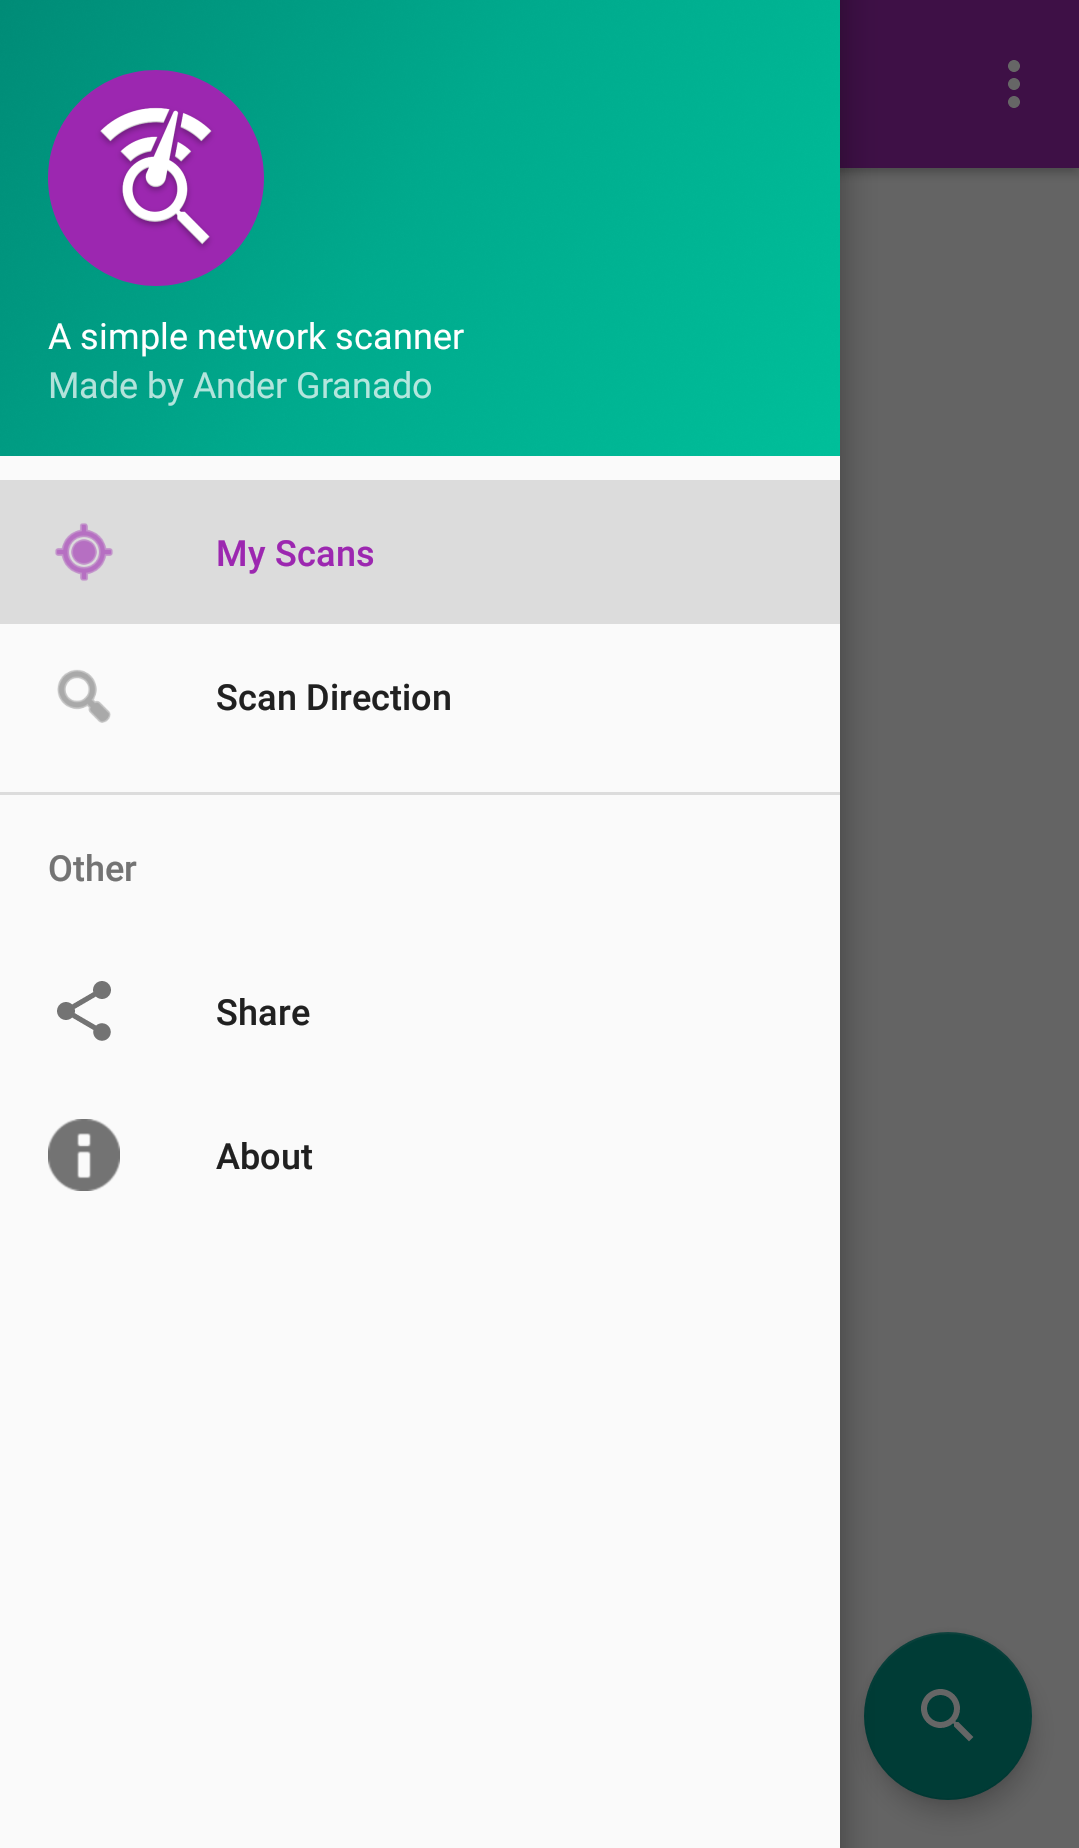
\includegraphics[width=0.5\textwidth]{navbar}
	\caption{Navbar principal de la aplicación}
	\label{fig:navbar}
\end{figure}

Se puede elegir entre una de las cuatro opciones y la opción seleccionada se mostrará marcada.

\subsection{Escaneos de red}

Como se ha mencionado, dentro de esas cuatro opciones, la que se muestra por defecto es \textbf{ScanListFragment}. Esta opción mostrará los diferentes escaneos realizados en una lista con una interfaz clara y simple, como se aprecia en la \autoref{fig:scanListFragment}.

\begin{figure}[H] % TODO: Cambiar la imagen por la de verdad
	\centering
	
\includegraphics[width=0.5\textwidth]{placeholder}
	\caption{Diseño de ScanListFragment para mostrar los diferentes escaneos realizados}
	\label{fig:scanListFragment}
\end{figure}

Dentro de esta interfaz también tendremos un elemento básico importante dentro de la aplicación, qué es el botón que encontramos en la parte inferior derecha. Este botón, o mejor dicho, \textit{Floating Action Button}, es un elemento que funciona de la misma manera que lo haría un botón corriente, pero con la particularidad de que se encuentra flotando por encima de la interfaz, lo que quiere decir que su posición es siempre fija, independientemente de si vamos descendiendo por la lista de escaneo realizados.

Pulsando este botón lograremos ejecutar la funcionalidad principal de la aplicación, que consiste en escanear una red. Tal y como muestra el diagrama, para escanear una red se abre otra Activity, llamada \textbf{NetworkScanActivity}.

Por lo tanto desde aquí tendremos dos opciones. La primera, pulsar sobre un escaneo ya realizado, lo que nos abrirá un Activity, llamada \textbf{NodeListActivity}, que se encarga de mostrarnos los nodos para ese escaneo en concreto. La segunda consiste en pulsar el FAB, lo que iniciará el escaneo de la red y abrirá otra Activity llamada \textbf{NetworkScanActivity}.

En el propio diagrama se observa que, aunque cada una de esas dos opciones abren una Activity diferente, ambas van a representar su interfaz gráfica mediante el mismo Fragment, el \textbf{NodeListFragment}. Aquí es donde se nota el potencial de los Fragments, que nos permiten reutilizar implementación de la parte gráfica en diferentes puntos de la aplicación, como se muestra en la \autoref{fig:nodeListFragmentDifference}.

\begin{figure}[H] % TODO: Cambiar la imagen por la de verdad
	\centering
	
\includegraphics[width=0.5\textwidth]{placeholder}
	\caption{Diferencia en NodeListFragment para un escaneo guardado y uno en curso}
	\label{fig:nodeListFragmentDifference}
\end{figure}

Tenemos que tener en cuenta que, en caso de hacer un escaneo de una red, aparte de realizar el escaneo, queremos mostrar los nodos en una lista los nodos que vayamos obteniendo. En caso de querer visualizar un escaneo ya hecho queremos mostrar también una lista de nodos. La funcionalidad para mostrar una lista de nodos se implementa un único Fragment, de tal manera que, aunque las dos operaciones a realizar sean diferentes, comparten la forma de visualizar los datos. Por ello, la parte correspondiente a cada caso particular se implementa dentro de sus respectivos Activities, mientras que la visualización de la lista de nodos se implementa directamente en el Fragment.

Después (en ambas opciones), en caso de seleccionar un nodo concreto, se mostrará información sobre ese nodo, independientemente de que sea un escaneo ya guardado o el escaneo que acabamos de realizar. Para lograr esto, simplemente se enlaza a otra Activity llamada \textbf{NodeInfoActivity}, mostrada a continuación.

\begin{figure}[H] % TODO: Cambiar la imagen por la de verdad
	\centering
	
\includegraphics[width=0.5\textwidth]{placeholder}
	\caption{Diseño del NodeInfoActivity}
	\label{fig:nodeInfoActivity}
\end{figure}

En esta Activity se muestra la información obtenida. Información como la dirección IP,  la dirección de hardware, el nombre del host, el fabricante o una tabla que muestra los diferentes servicios que tiene accesibles, con sus respectivos puertos, protocolos e información asociada.

\subsection{Escaneos de host}

De esas opciones, la otra que también resulta de interés es la que podremos usar para analizar una dirección concreta, que se muestra en \autoref{fig:scanDirectionFragment} y está implementada en el Fragment \textbf{ScanDirectionFragment}.

\begin{figure}[H] % TODO: Cambiar la imagen por la de verdad
	\centering
	
\includegraphics[width=0.5\textwidth]{placeholder}
	\caption{Diseño del ScanDirectionFragment}
	\label{fig:scanDirectionFragment}
\end{figure}

Una vez accedemos a él, vemos que su interfaz también es muy sencilla. Está compuesta solamente de tres elementos. El primero es un campo de texto donde podremos introducir la dirección IP o el dominio del nodo host que queramos analizar. El segundo nos permite elegir el modo de escaneo. Como se puede observar, tenemos cinco modos diferentes que influyen en la cantidad de información que podremos obtener. Obviamente, cuanto más exhaustivo sea el modo de escaneo, más tiempo va a tardar aplicación en analizar dicho nodo.

Una vez terminado el escaneo del host se abrirá otra Activity, llamada DirectionScanActivity,  que nos muestra la información del host escaneado, como se puede ver en la \autoref{fig:directionScanActivity}. En este caso la información se muestra de manera diferente a la información de un nodo de una red. Tenemos otra vista, esta vez separada en diferentes pestañas. Estas tres pestañas contienen partes de la información obtenida.

La primera de ellas, implementada en el \textbf{BasicInfoFragment}, simplemente muestra información con la dirección IP y el nombre del dominio. La segunda, llamada \textbf{ServicesInfoFragment}, muestra la información de los diferentes servicios abiertos en dicho host. La tercera y última, llamada \textbf{ExtraInfoFragment}, muestra información extra, como por ejemplo el tiempo de escaneo o el número de host detectados.

\begin{figure}[H] % TODO: Cambiar la imagen por la de verdad
	\centering
	
\includegraphics[width=0.5\textwidth]{placeholder}
	\caption{Diseño del DirectionScanActivity y sus tres pestañas}
	\label{fig:directionScanActivity}
\end{figure}

Cabe destacar que, por diversos motivos, se ha diferenciado entre la visualización de la información de un nodo de una red y la información de un host concreto que queramos analizar. El primero de ellos es que podemos tener diferentes objetivos a la hora de examinar los nodos que tenemos en nuestra red inalámbrica o examinar la información de un solo dominio. Al haber implementado la interfaz gráfica de manera diferente, podremos en un futuro ampliar la funcionalidad del escaneo del host para que muestre otros aspectos más complejos, sin con ello afectar a la información que se muestra de un nodo.

\section{Aspectos gráficos de Material Design}

Hasta ahora se han ido analizando individualmente cada Activity y Fragment y mostrando sus relaciones entre ellos. Además, se han ido mostrando imágenes del aspecto de cada uno de ellos. En dichas imágenes se han podido apreciar ciertos aspectos de la interfaz gráfica, aspectos en los que merece la pena indagar para explicar cómo y porqué se han implantado de esa manera.

\subsection{Color}

El primero de ellos es el color: en las imágenes mostradas se ha podido observar que en la interfaz existe, aparte del blanco, dos colores principales. Estos colores no son una elección arbitraria y además guardan relación entre ellos.

La elección de colores dentro de Material Design está acotada una cierta paleta \cite{mat-des-color}, que permite que los colores mostrados sean lo más agradables a la vista posible. A la hora de desarrollar una aplicación se han de elegir como mínimo dos colores. Los que se denominaría como color primario y color secundario, respectivamente. Para estos dos colores no podremos elegir cualquier color, sino una serie de valores concretos dentro de una paleta.

Dentro de esa paleta existe una manera concreta de especificar la claridad u oscuridad de un color en concreto. Se utilizan valores fijos que van desde el 900 hasta el 50, como se muestra para un color arbitrario en la \autoref{fig:material-design-color}.

\begin{figure}[H]
	\centering
	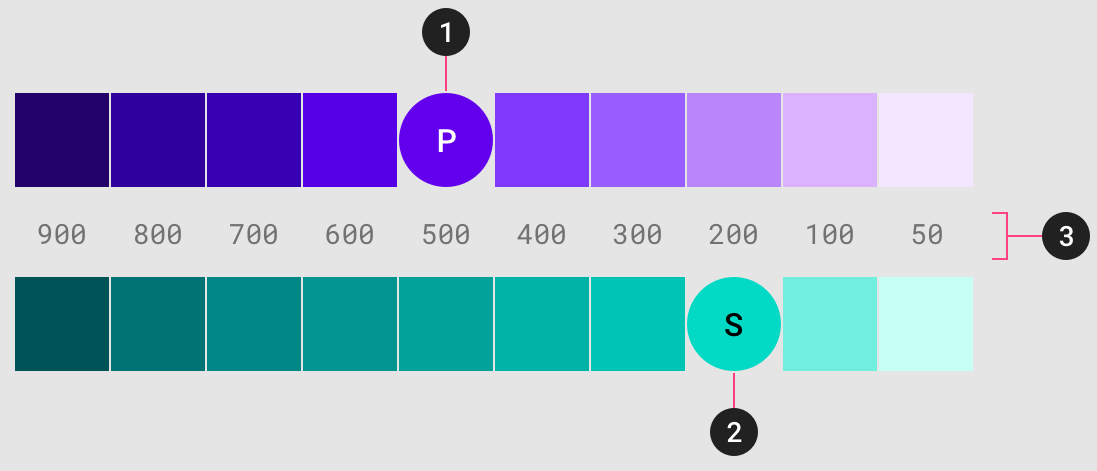
\includegraphics[width=0.7\textwidth]{material-design-color}
	\caption{Ejemplo de distinción de colores primario y secundario en Material Design}
	\label{fig:material-design-color}
\end{figure}

A medida que el número aumenta, el color se vuelve más oscuro. Cada color concreto de Material Design tiene toda esta gama de rangos disponibles para elegir. Lo que Material Design recomienda es elegir un color principal con una tonalidad 500 y un color secundario con una tonalidad de entre 500 a 200. Además estos dos colores no pueden ser cualquiera, sino que lo recomendable sería que de alguna manera fueran complementarios.

En base a todo lo mencionado se han elegido los colores \textit{Purple} y \textit{Teal} tan característicos de la aplicación (ver \autoref{fig:material-design-color-election}). Además también se ha elegido un color de énfasis para el color principal, que se utiliza en algunos puntos concretos de la aplicación.

\begin{figure}[H]
	\centering
	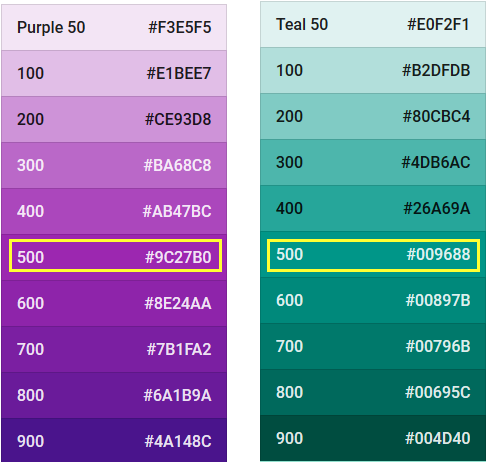
\includegraphics[height=0.4\textheight]{material-design-color-election}
	\caption{Colores finales elegidos para la aplicación}
	\label{fig:material-design-color-election}
\end{figure}

Los códigos hexadecimales de los colores están definidos en \mintinline{kotlin}{colors.xml}, qué es el archivo que se utiliza en Android para definir los colores y tenerlos accesibles desde cualquier parte de nuestra aplicación.

\begin{figure}[H]
	\centering
	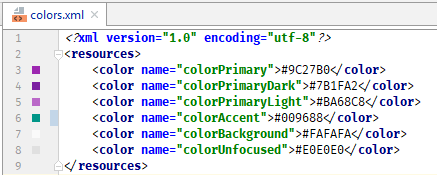
\includegraphics[width=0.8\textwidth]{colors-xml}
	\caption{Definición de los colores en el fichero colors.xml del proyecto en Android Studio}
	\label{fig:colors-xml}
\end{figure}

Por último en lo que al color se refiere, destacar que, en caso de haber usado el fondo claro (en este caso blanco) el texto mostrado se dibuja, o bien en negro, o en tonalidades de gris oscuro. Y al contrario, en caso de haber un color oscuro (en este caso el color principal) los elementos de texto se escriben en blanco. Esto permite que los diferentes textos mostrados en la aplicación sean claramente legibles.

\subsection{Layout}

Otro de los elementos importantes a la hora de diseñar la aplicación ha sido la distribución de elementos en ella, o lo que se conoce en inglés cómo \textit{layout}. Ws muy importante distribuir estos elementos correctamente por varios motivos.

El primero de ellos es la sensación que puede dar al usuario en la interfaz. Si tenemos los elementos agrupados en un espacio muy concreto, con poca separación o márgenes, daremos una sensación de  sobrecarga y al usuario le resultará más difícil comprender la aplicación. Si los tenemos desordenados dificultará también su uso. Es necesario colocarlos ordenados y especiados correctamente en pro de ofrecer al usuario la información de la manera más clara posible

Por otra parte, el uso de márgenes concretos estandarizados y programados de tal manera que se adapten a cualquier tipo de pantalla, hará que nuestra aplicación se vea bien independientemente de la pantalla del dispositivo que la esté ejecutando.

Durante toda la aplicación se han utilizado márgenes concretos y dinámicos. Para especificar en Android distancias, como puede ser por ejemplo la distancia de un margen,  se usan una serie de medidas llamadas \textit{dp}. Estas medidas lo que hacen es modificarse en función del tamaño de la interfaz especificado en el dispositivo. Es decir, van a aumentar o a decrecer en función de que se activen o no ciertos parámetros de accesibilidad en el sistema, o se cambien cosas como el tamaño de textos.

Utilizando estas medidas, y no medidas absolutas como pueden ser los píxeles, haremos que independientemente de esas características, activadas o desactivadas en un dispositivo u otro, nuestra aplicación se adapte sin ningún tipo de problema.

Además se han utilizado solamente ciertos valores estándar dentro de las interfaces gráficas en Android. En este caso, los únicos valores que se han utilizado, tanto a la hora de definir márgenes como a la hora de definir el tamaño de un elemento, son distancias en \textit{dp} que sean múltiplos de 8, como pueden ser: 8dp, 16dp, 32dp, 48dp. Esto da una sensación de consistencia y unidad a los márgenes.

Por otra parte en lo que a interfaz adaptativa o diseño responsive se refiere, se ha hecho uso de ciertos tipos de layout concretos que implementan las Activities de Android. A la hora de añadir elementos en un Activity de Android, estos deben ser añadidos a un layout. Un layout está compuesto de uno o más elementos, como pueden ser campos de texto, botones o también otros layouts. De esta manera se construyen interfaces gráficas que tienen diferentes apartados o secciones, dentro de las cuales tienen agrupaciones de elementos diferentes. Según el tipo de layout que se utilice, este ordenará los elementos de una manera u otra.

En concreto, se ha hecho uso del \textit{ConstraintLayout} y del \textit{LinearLayout}.

\subsubsection{ConstraintLayout}

El ConstraintLayout es un tipo de layout que permite definir una jerarquía concreta a la hora de distribuir los elementos. Es decir, cada elemento estará relacionado y tendrá unos márgenes concretos en función de otros elementos. De esta manera podemos, por ejemplo, poner que un elemento este separado a una distancia concreta por debajo de otro elemento. Por lo tanto si el segundo elemento se mueve debido a un cambio, la interfaz este primero actuará en consecuencia.

Android Studio tiene una herramienta que permite definir de manera sencilla mediante un editor de este tipo de distribución de elemento. A fin de cuentas, el layout de un Activity no es más que un fichero XML que podemos modificar a mano, pero mediante esta herramienta que Android Studio provee, podremos editar dicho archivo XML pero interactuando de manera gráfica con la interfaz.

Para mostrar un ejemplo de como se ha implementado este layout, se va a usar el ejemplo del \textbf{NodeInfoActivity}. Los diferentes elementos que componen dicha Activity se muestran en la \autoref{fig:node-info-elements}.

\begin{figure}[H]
	\centering
	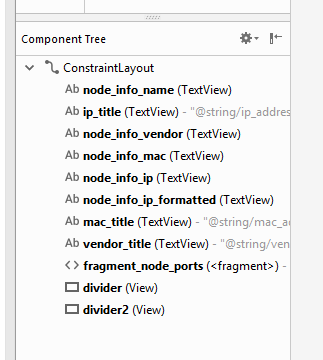
\includegraphics[height=0.4\textheight]{node-info-elements}
	\caption{Elementos del ConstraintLayout del NodeInfoActivity}
	\label{fig:node-info-elements}
\end{figure}

En dicha imagen se muestra una sección del editor de interfaces de Android Studio. En esa sección es donde podremos observar los diferentes elementos y la jerarquía de dichos elementos. Como se muestra, tenemos un layout de tipo ConstraintLayout y, dentro de él, diferentes elementos. Tenemos campos de texto para mostrar diferentes tipos de información, otros campos de texto que simplemente muestran nombres e incluso elementos más complejos, como barras de división o directamente otro Fragment entero, incrustado dentro de la Activity, que se encuentra al mismo nivel que el resto de elementos.

Anteriormente se ha mostrado una imagen sobre cómo se muestra la información de un nodo usando el \textbf{NodeInfoActivity}. Mientras que dicha imagen corresponde a la aplicación en ejecución, si entramos en el diseñador de interfaces gráficas de Android Studio, la imagen que obtendremos es diferente, como podemos observar en la \autoref{fig:android-studio-ui-editor}. En este caso tendremos dos vistas diferentes, la vista de diseño y la vista de blueprint. 

La vista de diseño, que es la de la izquierda, nos permite hacernos una idea de cómo se van a visualizar los elementos en nuestra aplicación (aunque debemos tener en cuenta que no es del todo exacta, ya que muchos de los elementos se cargarán o modificarán mediante código y, en este caso, lo único que estamos haciendo es mostrar los elementos del XML correspondiente).

La segunda vista, la de blueprint, nos permite trabajar sin distracciones sobre ciertas propiedades de los elementos, como pueden ser los márgenes, los tamaños o qué elementos están enlazados con otros.

\begin{figure}[H]
	\centering
	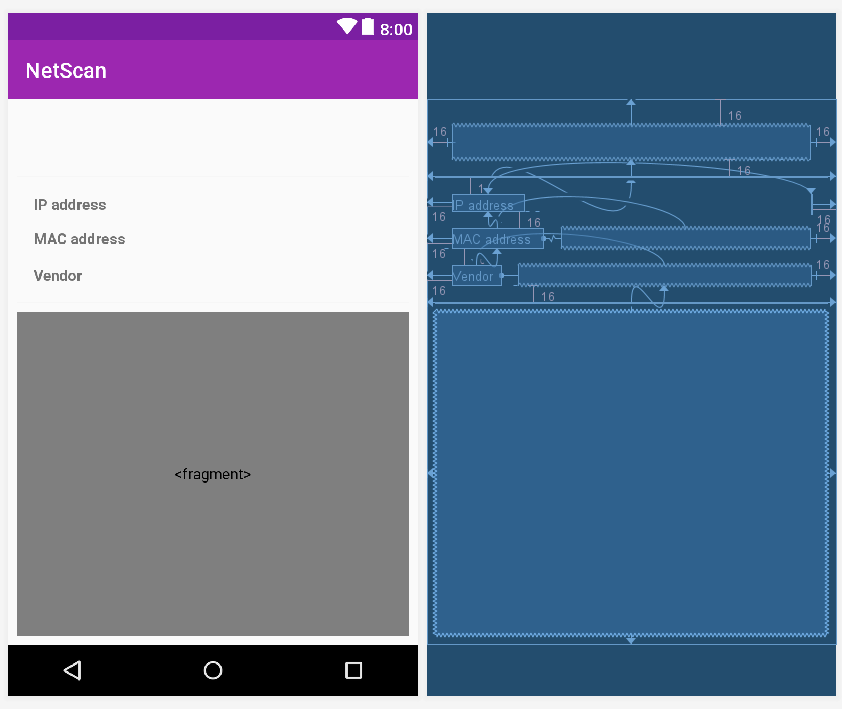
\includegraphics[height=0.4\textheight]{android-studio-ui-editor}
	\caption{Vistas de diseño y de blueprint del editor de interfaces gráficas de Android Studio}
	\label{fig:android-studio-ui-editor}
\end{figure}

En este caso vamos a hacer énfasis en el modo blueprint de parte de esa interfaz, que nos permitirá examinar el tamaño que ocupan los elementos y la relación entre ellos, sin tener las distracciones de los propios elementos. 

\begin{figure}[H]
	\centering
	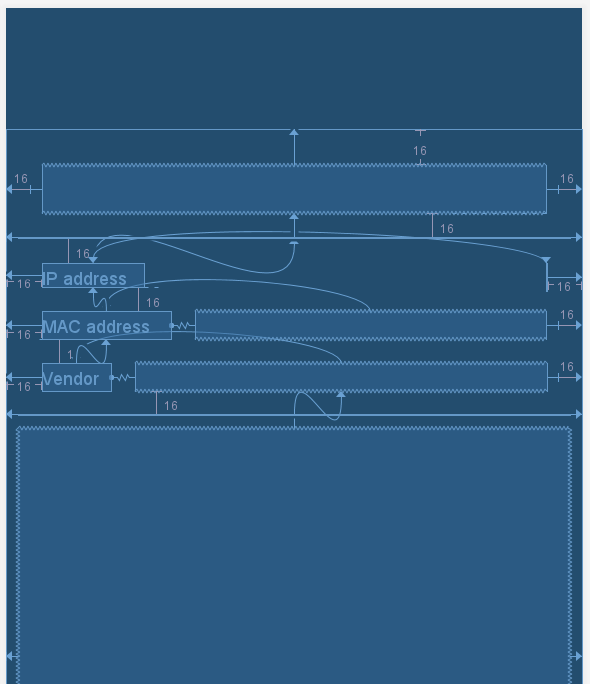
\includegraphics[width=0.6\textwidth]{android-studio-ui-blueprint}
	\caption{Layout y márgenes en un blueprint del NodeInfoActivity}
	\label{fig:ui-blueprint}
\end{figure}

El blueprint de la \autoref{fig:ui-blueprint} muestra una serie de flechas que básicamente indican qué elementos están relacionados con que otros. Podemos distinguir un primer elemento que tiene un margen de 16dp con respecto al borde superior. En base a ese elemento se van uniendo el resto de elementos, de tal manera que en caso de ampliarse algún tipo de elemento el resto de elementos se moverán en consonancia, ya que están enlazados unos con otros. A su vez, cada uno de los diferentes elementos tiene márgenes tanto a la izquierda como a la derecha. Estos márgenes, todos de 16dp, permiten que, independientemente del tamaño de la pantalla, tengamos los elementos perfectamente distribuidos.

Mediante el uso de márgenes con medidas concretas y enlazando los elementos con las opciones que nos permite el ConstraintLayout, nos queda una interfaz clara y completamente adaptativa, pudiéndose visualizar perfectamente independientemente de la pantalla.

\subsubsection{LinearLayout}

El segundo layout utilizado en la aplicación es el LinearLayout. Este layout, como bien su nombre indica, nos permitirá distribuir elementos de manera lineal. Esto lo podemos hacer tanto en vertical como en horizontal. En este caso, se ha utilizado en formato vertical y principalmente para mostrar listas de escaneos y de nodos, en los Fragments \textbf{ScanListFragment} y \textbf{NodeListFragment}. 

La gran ventaja del uso de este layout reside en que al añadir elementos al layout se irán posicionando automáticamente en vertical o en horizontal, formando una lista, por lo que podremos añadir elementos de manera dinámica, es decir, mediante código sin preocuparnos por especificar nada con respecto a dónde se van a mostrar.

\subsection{Tipografía}

En lo que a la tipografía se refiere, se ha aplicado principios similares a otros aspectos. La tipografía utilizada es la que se usa por defecto en las aplicaciones Android, denominada \textit{Roboto}. Esta tipografía es clara, legible y se integra la perfección con el sistema Android, ya que es la fuente que este último utiliza.

A la hora de usar diferentes tamaños o establecer diferentes opciones para dicha fuente, solo se han realizado ligeras modificaciones. En los aspectos en los que se quiere destacar algún elemento, como puede ser por ejemplo la dirección IP en alguna de las vistas, se ha hecho uso, por una parte, de la tipografía en negrita y, por otra parte, del uso del color secundario para darle mayor visibilidad.

También se ha hecho uso de la tipografía en formato monoespaciado cuando se ha querido representar valores que siempre van a tener la misma longitud. Es por todos sabido que, por ejemplo, una dirección de hardware siempre tiene la misma longitud, y representarlo con la tipografía monoespaciada permite que siempre tenga el mismo tamaño el bloque de texto a mostrar. Se puede apreciar estos cambios en la \autoref{fig:typo-options}

\begin{figure}[H]
	\centering
	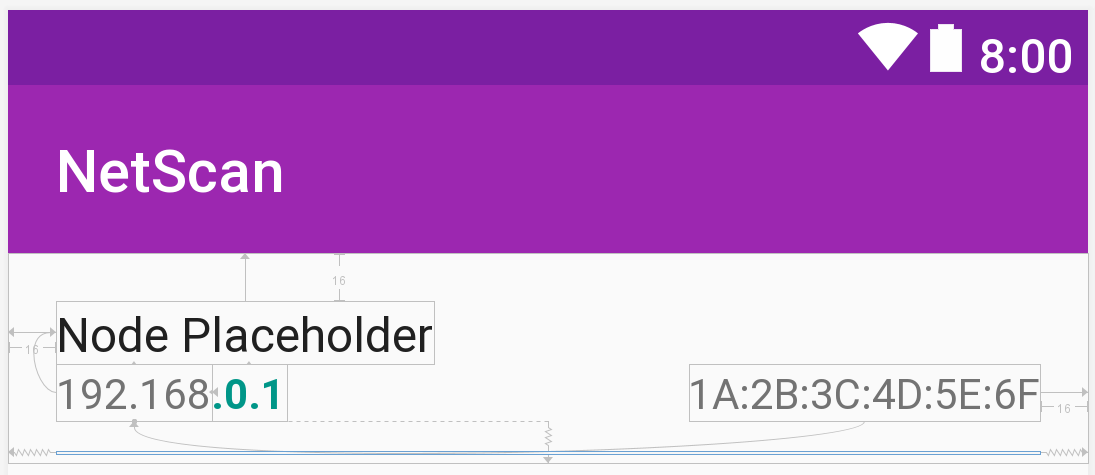
\includegraphics[width=0.7\textwidth]{typo-options}
	\caption{Diferentes opciones aplicadas a la tipografía original}
	\label{fig:typo-options}
\end{figure}

Por último con respecto a la tipografía, los tamaños utilizados siguen unos principios similares a los los utilizados para los márgenes. En este caso el sistema que se utiliza de medida no es el utilizado para las distancias, márgenes, que es el \textit{dp}, sino que se trata del \textit{sp}. Este sistema para dimensionar las tipografías que permite es que, si en el propio sistema cambiamos la tipografía para que sea de un tamaño superior e inferior, esta se adapte en función de dicho ajuste.

Durante toda la aplicación se ha mantenido en la mayor parte del texto los tamaños estándar (de 16sp), exceptuando algunas pequeñas ocasiones en las que se ha mostrado elementos con un tamaño mayor, siempre utilizando medidas definidas dentro del estándar de Material Design.

\subsection{Iconografía}

En una aplicación, la iconografía, junto a la tipografía y otros elementos de diseño, definen el estilo de la aplicación. Aunque es un área que abarca muchísimos campos del diseño y puede ser todo lo compleja que se quiera, para esta aplicación en concreto simplemente se han tenido en cuenta dos aspectos básicos.

El primero de ellos son los diferentes iconos usados para mostrar diferentes opciones, como pueden ser los usados en la barra de navegación o en los ajustes. Los iconos utilizados son los iconos estándar que se usan en Android. Esto, junto a los otros elementos, da una sensación de unidad mayor, ya que se asemejan estilo a los iconos del sistema de Android.

Por otro lado, está el icono de la propia aplicación. El icono de la aplicación es simple a más no poder. Está compuesto únicamente de la conjunción de dos de los iconos estándar de Android y el color principal. Estos dos iconos son el icono de la lupa, que represent una búsqueda de algún tipo, y el icono de la búsqueda de redes, que representa la búsqueda de una red. La conjunción de ambas representa el objetivo principal de la aplicación. Unido al color principal usado, logramos un icono sumamente sencillo, pero que encaja a la perfección con la aplicación. El icono se puede ver en la \autoref{fig:app-icon}.

\begin{figure}[H]
	\centering
	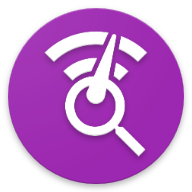
\includegraphics[width=0.15\textwidth]{app-icon}
	\caption{Icono de la aplicación en formato redondeado}
	\label{fig:app-icon}
\end{figure}

\section{Conclusiones}

El desarrollo de interfaces gráficas en Android y la aplicación de los principios de Material Design es un campo inmensamente amplio.Según qué aplicación se esté desarrollando, y de lo grande que sea, podemos encontrar perfiles concretos desarrolladores que invierten su trabajo únicamente en este aspecto, el de la interfaz gráfica y el de la experiencia de usuario. Es un campo que abarca muchas más áreas de las que se han cubierto en esta sección y el abarcar todos esos campos ya sería elemento suficiente para constituir un proyecto completamente independiente.

Lo que se ha querido mostrar en esta sección es que, aunque la aplicación desarrollada sea sumamente sencilla a nivel gráfico, se han seguido aplicando principios para mantener la consistencia han dicho interfaz. En este casos, principios de Material Design, que logran una interfaz más clara, ordenada y atractiva a la vista, además de adaptarse a los diseños de interfaces de otras aplicaciones de Google y del propio sistema de Android.

De esta manera, en caso de que en un posible trabajo futuro se quiere ampliar la funcionalidad de la aplicación, simplemente debemos continuar siguiendo estos principios de diseño, para tener una aplicación unificada, fácil de usar y lo más atractiva posible.

